\section{Инфляция}

Уровень инфляции по годам в Еврозоне, \%:

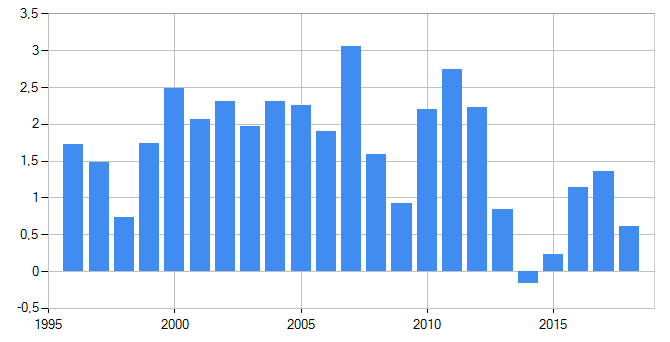
\includegraphics[width=16cm]{pics/alina/inflation.png}

Рассмотрим 3 варианта событий:

\begin{itemize}
	\item Низкий уровень - 0,7\%. Через 5 лет с учетом инфляции 700.000 евро будут эквивалентны 725.845 евро
	\item Средний уровень - 1,7\%. Через 5 лет с учетом инфляции 700.000 евро будут эквивалентны 761.558 евро.
	\item Высокий уровень - 3,1\%. Через 5 лет с учетом инфляции 700.000 евро будут эквивалентны 815.439 евро
\end{itemize}